\documentclass[]{article}
\usepackage{lmodern}
\usepackage{amssymb,amsmath}
\usepackage{ifxetex,ifluatex}
\usepackage{fixltx2e} % provides \textsubscript
\ifnum 0\ifxetex 1\fi\ifluatex 1\fi=0 % if pdftex
  \usepackage[T1]{fontenc}
  \usepackage[utf8]{inputenc}
\else % if luatex or xelatex
  \ifxetex
    \usepackage{mathspec}
  \else
    \usepackage{fontspec}
  \fi
  \defaultfontfeatures{Ligatures=TeX,Scale=MatchLowercase}
  \newcommand{\euro}{€}
\fi
% use upquote if available, for straight quotes in verbatim environments
\IfFileExists{upquote.sty}{\usepackage{upquote}}{}
% use microtype if available
\IfFileExists{microtype.sty}{%
\usepackage{microtype}
\UseMicrotypeSet[protrusion]{basicmath} % disable protrusion for tt fonts
}{}
\usepackage{hyperref}
\PassOptionsToPackage{usenames,dvipsnames}{color} % color is loaded by hyperref
\hypersetup{unicode=true,
            pdftitle={SODA POP : Robust online Partial Ordering Planning for real life applications},
            pdfauthor={Paper ID\#232},
            pdfborder={0 0 0},
            breaklinks=true}
\urlstyle{same}  % don't use monospace font for urls
\usepackage{listings}
\usepackage{graphicx,grffile}
\makeatletter
\def\maxwidth{\ifdim\Gin@nat@width>\linewidth\linewidth\else\Gin@nat@width\fi}
\def\maxheight{\ifdim\Gin@nat@height>\textheight\textheight\else\Gin@nat@height\fi}
\makeatother
% Scale images if necessary, so that they will not overflow the page
% margins by default, and it is still possible to overwrite the defaults
% using explicit options in \includegraphics[width, height, ...]{}
\setkeys{Gin}{width=\maxwidth,height=\maxheight,keepaspectratio}
\setlength{\parindent}{0pt}
\setlength{\parskip}{6pt plus 2pt minus 1pt}
\setlength{\emergencystretch}{3em}  % prevent overfull lines
\providecommand{\tightlist}{%
  \setlength{\itemsep}{0pt}\setlength{\parskip}{0pt}}
\setcounter{secnumdepth}{5}

\title{SODA POP : Robust online Partial Ordering Planning for real life
applications}
\author{Paper ID\#232}
\date{}
\usepackage{xcolor, listings}
\usepackage{latex/aaai}
\usepackage{times}
\usepackage{helvet}
\usepackage{courier}
\usepackage{algorithm}
\usepackage[noend]{algpseudocode}
\usepackage{amsthm}

% We now define the sixteen \solarized{} colors.
\definecolor{solarized-base03} {RGB}{000, 043, 054}
\definecolor{solarized-base02} {RGB}{007, 054, 066}
\definecolor{solarized-base01} {RGB}{088, 110, 117}
\definecolor{solarized-base00} {RGB}{101, 123, 131}
\definecolor{solarized-base0}  {RGB}{131, 148, 150}
\definecolor{solarized-base1}  {RGB}{147, 161, 161}
\definecolor{solarized-base2}  {RGB}{238, 232, 213}
\definecolor{solarized-base3}  {RGB}{253, 246, 227}
\definecolor{solarized-yellow} {RGB}{181, 137, 000}
\definecolor{solarized-orange} {RGB}{203, 075, 022}
\definecolor{solarized-red}    {RGB}{220, 050, 047}
\definecolor{solarized-magenta}{RGB}{211, 054, 130}
\definecolor{solarized-violet} {RGB}{108, 113, 196}
\definecolor{solarized-blue}   {RGB}{038, 139, 210}
\definecolor{solarized-cyan}   {RGB}{042, 161, 152}
\definecolor{solarized-green}  {RGB}{133, 153, 000}

\newtheorem{definition}{Definition}

%%%%%% for algorithms
\errorcontextlines\maxdimen
\algrenewcommand\alglinenumber[1]{\tiny\color{solarized-base0} #1}

% begin vertical rule patch for algorithmicx (http://tex.stackexchange.com/questions/144840/vertical-loop-block-lines-in-algorithmicx-with-noend-option)
\makeatletter
% start with some helper code
% This is the vertical rule that is inserted
    \newcommand*{\algrule}[1][\algorithmicindent]{\makebox[#1][l]{\color{solarized-base0}\hspace*{.5em}\thealgruleextra\vrule height \thealgruleheight depth \thealgruledepth}}%
% its height and depth need to be adjustable
\newcommand*{\thealgruleextra}{}
\newcommand*{\thealgruleheight}{.75\baselineskip}
\newcommand*{\thealgruledepth}{.25\baselineskip}

\newcount\ALG@printindent@tempcnta
\def\ALG@printindent{%
    \ifnum \theALG@nested>0% is there anything to print
        \ifx\ALG@text\ALG@x@notext% is this an end group without any text?
            % do nothing
        \else
            \unskip
            \addvspace{-1pt}% FUDGE to make the rules line up
            % draw a rule for each indent level
            \ALG@printindent@tempcnta=1
            \loop
                \algrule[\csname ALG@ind@\the\ALG@printindent@tempcnta\endcsname]%
                \advance \ALG@printindent@tempcnta 1
            \ifnum \ALG@printindent@tempcnta<\numexpr\theALG@nested+1\relax% can't do <=, so add one to RHS and use < instead
            \repeat
        \fi
    \fi
    }%
\usepackage{etoolbox}
% the following line injects our new indent handling code in place of the default spacing
\patchcmd{\ALG@doentity}{\noindent\hskip\ALG@tlm}{\ALG@printindent}{}{\errmessage{failed to patch}}
\makeatother

% the required height and depth are set by measuring the content to be shown
% this means that the content is processed twice
\newbox\statebox
\newcommand{\myState}[1]{%
    \setbox\statebox=\vbox{#1}%
    \edef\thealgruleheight{\dimexpr \the\ht\statebox+1pt\relax}%
    \edef\thealgruledepth{\dimexpr \the\dp\statebox+1pt\relax}%
    \ifdim\thealgruleheight<.75\baselineskip
        \def\thealgruleheight{\dimexpr .75\baselineskip+1pt\relax}%
    \fi
    \ifdim\thealgruledepth<.25\baselineskip
        \def\thealgruledepth{\dimexpr .25\baselineskip+1pt\relax}%
    \fi
    %\showboxdepth=100
    %\showboxbreadth=100
    %\showbox\statebox
    \State #1%
    %\State \usebox\statebox
    %\State \unvbox\statebox
    %reset in case the next command is not wrapped in \myState
    \def\thealgruleheight{\dimexpr .75\baselineskip+1pt\relax}%
    \def\thealgruledepth{\dimexpr .25\baselineskip+1pt\relax}%
}
% end vertical rule patch for algorithmicx


%%%% For listings (code blocks)
\lstset{
    basicstyle={\footnotesize\ttfamily},
    numbers=left,
    keywordstyle=\color{solarized-orange}\bfseries,
%    identifierstyle=\color{solarized-base02},
    stringstyle=\color{solarized-cyan},
    commentstyle=\color{solarized-base1}\itshape,
    numberstyle=\tiny\color{solarized-base0},
    columns=flexible,
    stepnumber=1,
    numbersep=5pt,
    backgroundcolor=\color{solarized-base3},
    showspaces=false,
    showstringspaces=false,
    showtabs=false,
    tabsize=2,
    captionpos=b,
    breaklines=true,
    breakatwhitespace=true,
    breakautoindent=true,
    escapeinside={\%*}{*)},
    linewidth=\textwidth,
    basewidth=0.5em,
}


%%%% For links URL
\hypersetup{colorlinks=true, linkcolor=solarized-blue, citecolor=solarized-base1, filecolor=solarized-magenta, urlcolor=solarized-cyan}

% Redefines (sub)paragraphs to behave more like sections
\ifx\paragraph\undefined\else
\let\oldparagraph\paragraph
\renewcommand{\paragraph}[1]{\oldparagraph{#1}\mbox{}}
\fi
\ifx\subparagraph\undefined\else
\let\oldsubparagraph\subparagraph
\renewcommand{\subparagraph}[1]{\oldsubparagraph{#1}\mbox{}}
\fi

\begin{document}
\maketitle
\begin{abstract}
As of recent years, automated planning domain has mainly focused on
performances and advances in state space planning to improve
scalability. That orientation shadows other less efficient ways of doing
like Partial Ordering Planning (POP) that has the advantage to be much
more flexible. This approach \emph{generates} plans that can be refined
easily and can be used to achieve greater resilience, repairing
capabilities and soft resolution that applications \emph{based on}
online plan recognition or decision-making can benefit from. \emph{This
paper presents} a set of algorithms, named Soft Ordering and Defect
Aware Partial Ordering Planning (SODA POP), that aims at targeting these
objectives and maintain a high plan quality. Our algorithms create
proper offline plans for goals and use an effective defect fixing
\emph{algorithm} to repair input plans even if these plans are
corrupted. SODA POP can also use healer actions and links in order to
always return a valid plan even in cases where the problem is impossible
to solve using problem derivation. Some relevant properties of these
algorithms are analyzed in this article and experimental results show
interesting performances for online planning and repairing.
\end{abstract}

\section*{Introduction}\label{introduction}
\addcontentsline{toc}{section}{Introduction}

For some time Partial Order Planning (POP) has been the most popular
approach to planning resolution. This kind of algorithms are based on
\emph{least commitment strategy} on plan step ordering that can allow
actions to be flexibly interleaved during execution {[}1{]}. Thus, the
way the search is made using flexible partial plan as a search space
allowed for more versatility for a wide variety of uses. As of more
recent years, new state space search models and heuristics {[}2{]} have
been demonstrated to be more efficient than POP planners due to the
simplicity and relevance of states representation opposed to partial
plans {[}3{]}. This have made the search of performance the main axis of
research for planning in the community .

While this goal is justified, it shadows other problems that some
practical applications cause. For example, the flexibility of Plan Space
Planning (PSP) is an obvious advantage for applications needing online
planning: plans can be repaired on the fly as new informations and
objectives enter the system. The idea of using POP for online planning
and repairing plans instead of replanning everything is not new {[}4{]},
but has never been paired with the resilience that some other cognitive
applications may need, especially when dealing with sensors noise in
input data.

This resilience makes fixing errors easier than with an external
algorithm as the plan logic allows for context driven decision on the
way to repair the issues. For example if an action becomes unrelevant or
incoherent, the flaw in the partial plan makes the issue explicit and
therefore easier to fix. Softwares might sometimes provide plans that
can contain errors and imperfections that will decrease significantly
the efficiency of the computation and the quality of the output plan.

Adding to that, these plans may become totally unsolvable. This problem
is to our knowledge not treated in planning of all forms (state
planning, PSP, and even constraint satisfaction planning) as usually the
aim is to find a solution relative to the original plan (which makes
sense). But as we proceed a mechanism of \emph{problem derivation} may
be required. This will allow soft solving of any problem regardless of
its resolvability.

One of the applications that needs these improvements is plan
recognition with the particular use of off-the-shelf planners to infer
the pursued goal of an agent where online planning and resilience is
particularly important {[}5{]}. This method adds dummy actions that need
to be satisfied by modifying the goal to ensure that the observed plan
is selected by the planner. A system that is able to repair plan in real
time will ease such an application. Another application is
decision-making in dynamical environments. Indeed, having a plan that
details all steps and explicits the ones that are not possible, can help
decide of the plan of action to take.

These problems call for new ways to improve the answer of a planner.
These improvements must provide relevant plan information pointing out
exactly what needs to be done in order to make a planning problem
solvable, even in the case of obviously inconsistent input data. This
paper aims to solve this while preserving the advantages of PSP
algorithms (flexibility, easy fixing of plans, soundness and
completeness). Our Soft Ordering and Defect Aware Partial Ordering
Planning (SODA POP) algorithm will target those issues.

Our new set of auxiliary algorithms allows making POP algorithm more
resilient, efficient and relevant. This is done by pre-emptively
computing proper plans for goals, by solving new kinds of defects that
input plans may exhibit, and by healing compromised plan by deriving the
initial problem with forged actions to allow resolution.

To explain this work we first introduce a few notions, notations and
specificities of existing POP algorithms. Then we present and illustrate
their limitations, categorizing the different defects arising from the
resilience problem and explaining our auxiliary algorithms, their uses
and properties. To finish we compare the performance, resilience and
quality of POP and our solution.

\section{Definitions}\label{definitions}

First we introduce some definitions and notations for mathematical
representation to present our model.

\subsection{Classical planning}\label{classical-planning}

\begin{definition}[Fluents]

A fluent is a property of the world. We note \(\lnot f\) the
complementary fluent of \(f\) meaning that \(f\) is true when
\(\lnot f\) is false and vice-versa.

\end{definition}

It is often represented by first order logical propositions but in this
paper we choose to focus on the algorithm and to represent fluents as
simple literals (fully instantiated) using \(\mathbb{Q}^*\), the set of
relative integers without \(0\), as the fluent domain. We use negative
integers to represent opposite fluents.

\begin{definition}[State]

A state is defined as a set of fluents. States can be additively
combined. We note
\(s_1 + s_2 = \left( s_1 \cup s_2 \right) - \left\{ f \middle| f \in s_1 \land \lnot f \in s_2 \right\}\)
such operation. It is the union of the fluents with an erasure of the
complementary ones.

\end{definition}

\begin{definition}[Action]

An action is a state operator. It is represented as a tuple
\(a = \langle pre, eff \rangle\) with \(pre\) and \(eff\) being sets of
fluents, respectively the preconditions and the effects of \(a\). An
action can be used only in a state that verifies its preconditions. We
note \(s \models a \Leftrightarrow pre(a) \subset s\) the verification
of an action \(a\) by a state \(s\).

\end{definition}

An action \(a\) can be functionally applied to a state \(s\) as follows
: \[a:= \substack{ \left\{ s \models a \middle| s \in S\right\} \to S\\
    a(s) \mapsto s + eff(a)}\] with \(S\) being the set of all states.
This means that an action adds all its effect to the state of the world
on application (by removing complementary fluents if needed)

We distinguish between two specific kinds of actions : actions with no
preconditions are synonymous to a state and those with empty effect are
called a goal.

\subsection{Plan Space Planning}\label{plan-space-planning}

\subsubsection{Problem}\label{problem}

We define a partial plan satisfaction problem as a tuple noted
\(P = \langle A, I, G, p \rangle\) with :

\begin{itemize}
\tightlist
\item
  \(I\) and \(G\) being the pseudo actions representing respectively the
  initial state and the goal.
\item
  \(p\) being a partial plan to refine.
\item
  \(A\) the set of all actions.
\end{itemize}

\begin{definition}[Partial Plan]

A \emph{partial plan} is a tuple \(p = \langle A_p, L\rangle\) where
\(A_p\) is a set of steps (actions) and \(L\) is a set of causal links
of the form \(a_i \xrightarrow{f} a_j\), such that
\(\{ a_i, a_j \} \subset A_p \land f \in eff(a_i) \cap pre(a_j)\) or
said otherwise, this causal link means that the fluent \(f\) is provided
by an effect of \(a_i\) to a precondition of \(a_j\). We include the
ordering constraints of PSP in the causal links. An ordering constraint
is noted \(a_i \to a_j\) and means that the plan means \(a_i\) as a step
that is prior to \(a_j\) without specific cause (usually because of
threat resolution). We note the order relation over \(A\) for an action
\(a_i\) that is prior to the action \(a_j\) following all the causal
links and ordering constraints \(a_i \succ a_j\) .

\end{definition}

The figure \ref{fig:legend} details how the elements of partial plans
are represented in the rest of this paper.

\begin{figure}[htbp]
\centering
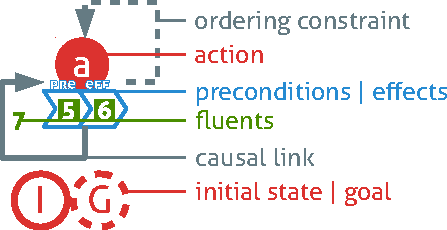
\includegraphics{graphics/legend.pdf}
\caption{Global legend for how partial plans are represented in this
paper\label{fig:legend}}
\end{figure}

In this figure the fluent \(5\) is a precondition of the action \(a\)
and the fluent \(6\) an effect. The causal link is providing the fluent
\(7\) (only as a representation example or it would be a liar link). The
dotted line is an ordering constraint that would mean that \(a\) should
be placed before \(a\) (for representation still or it would be a
cycle). \(I\) and \(G\) are respectively the initial and goal step.

\subsubsection{Flaws}\label{flaws}

When refining a partial plan, we need to fix flaws. Those could be
present in the input or created by the refining process. Flaws can
either be unsatisfied subgoals or threats to causal links.

\begin{definition}[Subgoal]

A subgoal \(s\) is a precondition of an action \(a_s \in A_p\) with
\(s \in pre(a_s)\) that isn't satisfied by any causal link. We can note
a subgoal as :
\[a_i \xrightarrow{s} a_s \notin L \mid \{ a_i, a_s \} \subset A_p \]

\end{definition}

\begin{definition}[Threat]

A step \(a_t\) is said to threaten a causal link
\(a_i \xrightarrow{t} a_j\) if and only if
\[\neg t \in eff(a_t) \land a_i \succ a_t \succ a_j \models L\]

\end{definition}

In other words, the action has a possible complementary effect that can
be inserted between two actions needing this fluent while being
consistent with the ordering constraint in \(L\).

\subsubsection{Resolvers}\label{resolvers}

Resolvers are a set of actions and causal links
\(r = \langle A_r , L_r \rangle\) that fixes flaws. A resolver for a
subgoal is an action \(a_r \in A\) that has \(s\) as an effect
\(s \in eff(a_r)\) inserted along with a causal link noted
\(a_r \xrightarrow{s} a_s\). The usual resolvers for a threat are either
\(a_t \to a_i\) or \(a_j \to a_t\) which are called respectively
promotion and demotion links. Another resolver is called a white knight
that is an action \(a_k\) that reestablishes \(t\) after \(a_t\) along
with an ordering constraint \(a_t \to a_k\) and a causal link
\(a_k \xrightarrow{t} a_j\).

\subsubsection{Solution}\label{solution}

The solution of a PSP problem is a valid partial plan that respect the
specification of said problem (only using actions in \(A\) and having
the correct initial and goal step).

\begin{definition}[Consistency]

A partial plan is consistent if it contains no ordering cycles. That
means that the directed graph formed by step as vertices and causal
links as edges isn't cyclical. This is important to guarantee the
soundness of the algorithm.

\end{definition}

\begin{definition}[Flat Plan]

We can instantiate one or several flat plans from a partial plan. A flat
plan is an ordered sequence of actions \(\pi = [ a_1, a_2 \ldots a_n]\)
that acts like a pseudo action
\(\pi = \langle pre_\pi, eff_\pi \rangle\) and can be applied to a state
\(s\) using functional composition operation
\(\pi := \bigcirc_{i=1}^n a_n\).

\end{definition}

We call a flat plan valid if and only if it can be functionally applied
on an empty state. We note that this is different from classic state
planning because in our case the initial state is the first action that
is already included in the plan.

\begin{definition}[Validity]

A partial plan is valid if and only if it is consistent and if all flat
plans that can be generated are valid.

\end{definition}

\section{Classical POP}\label{classical-pop}

Partial Order Planning (POP) is a popular implementation of the general
PSP algorithm. It refines a partial plan by trying to fix its flaws and
is proven to be sound and complete {[}6{]}.

\subsection{Description}\label{description}

\begin{algorithm}\caption{Classical Partial Order Planning}\label{pop}\begin{algorithmic}[1]

\Function{pop}{Queue of Flaws $agenda$, Problem $P$}
\State \Call{populate}{$agenda$, $P$} \Comment{Only on first call}
\If{$agenda = \emptyset$} \State \Return Success
\Comment{Stop all recursion} \EndIf
    \State Flaw \(f\gets agenda.pop\)
\Comment{First element of the queue} \State Resolvers \(R \gets\)
\Call{resolvers}{$f$, $P$} \Comment{Ordered list of resolvers to try}
\ForAll{$r \in R$} \Comment{Choice operator}
\State \Call{apply}{$r$, $P.p$} \If{\Call{consistent}{$P.p$}}
\State \Call{pop}{$agenda \cup$ \protect\Call{relatedFlaws}{$f$}, $P$}
\Else 
            \State \Call{revert}{$r$, $P.p$} \EndIf
    \EndFor
    \State \Return Failure \Comment{Return to last choice of resolver}
\EndFunction

\end{algorithmic}\end{algorithm}

Algorithm 1 presents the base algorithm for a planer in the plan space.
POP implementation uses an agenda of flaws that is efficiently updated
after each refinement of the plan. A flaw is selected for resolution and
we use a non deterministic choice operator to pick a resolver for the
flaw. The resolver is inserted in the plan and we recursively call the
algorithm on the new plan. On failure we return to the last non
deterministic choice to pick another resolver. The algorithm ends when
the agenda is empty or when there is no more resolver to pick for a
given flaw.

\subsection{Limitations}\label{limitations}

This standard way of doing have seen multiple improvements over
expressiveness like with UCPOP {[}7{]}, hierarchical task network to add
more user control over sub-plans {[}8{]}, cognition with defeasible
reasoning {[}9{]}, or speed with multiple ways to implement the popular
fast forward method from state planning {[}10{]}. However, all these
variants do not treat the problem of online planning, resilience and
soft solving.

Some other closer works like {[}4{]} treats the problem of online
planning by removing big chunks of the partial plan by identifying
incorrect trees in the plan. This along with a heuristic of choice of
unrefinemment strategies causes a heavy replanning of the problem even
if only one action needs removal. This also lead to an exponential
number of plan to consider. This is a big problem when trying to adapt a
plan with minimal changes due to replanning.

Indeed, all these problems can affect POP's performance and quality as
they can interfere with POP's inner working when the algorithm is able
to give an answer at all.

Before continuing, we present a simple example of classical POP
execution with the following problem. We have an initial state
\(I = \langle \emptyset , \{ 1, 2 \} \rangle\) and a goal
\(G = \langle \{ 3, 4, -5, 6 \}, \emptyset \rangle\) encoded as dummy
steps. We also introduce actions that are not steps yet but that are
provided by \(A\). The actions \(a \langle \{1\}, \{3,5\} \rangle\),
\(b \langle \{2\}, \{4\} \rangle\) and
\(c \langle \{5\}, \{6\} \rangle\) are normal actions that are useful to
achieve the goal. The actions \(n \langle \{-8, 7\}, \{-7, 8\} \rangle\)
and \(l \langle \{-7, 8\}, \{-8, 7\} \rangle\) are looping actions that
are meant to cause cycles. The action
\(t \langle \{4\}, \{-5\} \rangle\) is meant to be threatening to the
plan's integrity and will generate threats. We introduce
\(u \langle \{4\}, \emptyset \rangle\) and
\(v \langle \{4\}, \{4\} \rangle\) as toxic actions,
\(w \langle \{9\}, \{3\} \rangle\) as a dead-end action and
\(x \langle \{7\}, \{-2,2\} \rangle\) as a contradictory action. These
notions will be defined \protect\hyperlink{defects}{later}.

\begin{figure}[htbp]
\centering
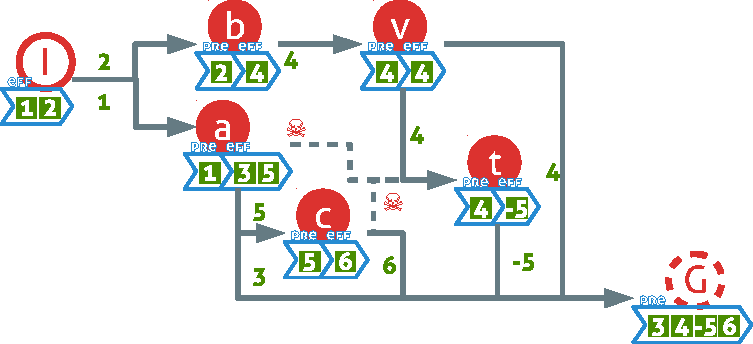
\includegraphics{graphics/pop.pdf}
\caption{Standard POP result to the problem\label{fig:pop}}
\end{figure}

This example has been crafted to illustrate problems with standard POP
implementations. We give a possible resulting plan of standard POP in
figure \ref{fig:pop}. We can see some issues as for how the plan has
been built. The action \(v\) is being used even if it is useless since
\(b\) already provided fluent \(4\). We can also notice that despite
being contradictory the action \(x\) raised no alarm. As for ordering
constraints, we can clearly see that the link \(a \to t\) is redundant
with the path \(a \xrightarrow{5} c \to t\) that already puts that
constraint by transitivity. Also, some problems arise during execution
with the selection of \(w\) that causes a dead-end.

Of course the flaw selection mechanism of certain variant can prevent
that to happen in that case. But often flaw selection mechanisms are
more speed oriented and will do little if a toxic action seems to fit
better than a more coherent but complex one .

All these issues are caused by what we call \emph{defects} as they are
not regular PSP flaws but they still cause problems with execution and
results. We will address these defects and propose a way to fix them in
\protect\hyperlink{defects}{the next section}.

\section{Auxiliary algorithms to POP}\label{auxiliary-algorithms-to-pop}

In order to improve POP algorithms' resilience, online performance and
plan quality, we propose a set of auxiliary algorithms that provides POP
with a clean and efficiently populated initial plan. The complete
algorithm will be presented in \protect\hyperlink{soda}{the next
section} as a combination of all auxiliary algorithms and classical POP.

\subsection{Proper plan generation}\label{proper-plan-generation}

\begin{algorithm}\caption{Proper plan generation for a given goal $g$}\label{properplan}\begin{algorithmic}[1]

\Function{properPlan}{Goal $g$, Actions $A$} \State Partial Plan
\(p \gets \emptyset\) \State Actions \(relevants \gets\)
\Call{satisfy}{$g$, $A$, $p$}
\Comment{Satisfy given goal with all necessary actions and causal links}
\State Queue of Actions \(open \gets relevants\)
\While{$open \neq \emptyset$} \State Action \(a\gets open.pop\)
\State Actions \(candidates \gets\) \Call{satisfy}{$a$, $A$, $p$}
\ForAll{$candidate \in candidates$} \If{$candidate \notin relevants$}
\State \(open.push(candidate)\) \EndIf
        \EndFor
    \EndWhile
\EndFunction

\end{algorithmic}\end{algorithm}

As in online planning goals can be known in advance, we propose a new
mechanism that generates proper plans for goals. We take advantage of
the fact that this step can be done offline to improve the performance
of online planning. This offline execution prevents us to access the
details of the initial state of the world as it will be defined at
runtime. We define for that the concept of \emph{participating action}.
An action \(a \in A\) participates in a goal \(G\) if and only if \(a\)
has an effect \(f\) that is needed to accomplish \(G\) or that is needed
to accomplish another participating action's preconditions. A proper
plan is a partial plan that contains all participating actions as steps
and causal links that bind them with the step they are participating in.
This proper plan is independent from the initial step because we might
not have the initial step at the time of the proper plan generation.

\begin{figure}[htbp]
\centering
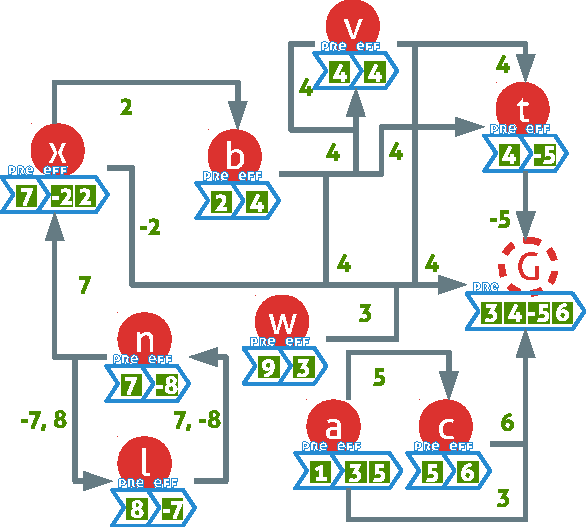
\includegraphics{graphics/proper.pdf}
\caption{Proper plan of the example goal\label{fig:proper}}
\end{figure}

We define the concept of \emph{participating action}. An action
\(a \in A\) participates in a goal \(G\) if and only if \(a\) has an
effect \(f\) that is needed to accomplish \(G\) or to accomplish another
participating action's preconditions. A proper plan is a partial plan
that contains all participating actions as steps and causal links that
bind them with the step they are participating in. Proper plan
generation, detailed in Algorithm 2, recursively chooses all
participating actions. It simply populate the proper plan with a quick
and incomplete backward chaining.

The partial plan doesn't have an initial state (because of its offline
nature). This auxiliary algorithm is therefore used as a caching
mechanism for online planning. The algorithm starts to populate the
proper plan with a quick and incomplete backward chaining.

Once applied on the example of figure \textbf{???}, proper plan
generation returns the partial plan presented in figure
\ref{fig:proper}. This partial plan doesn't have initial state because
of its offline nature. It also shows several cycles and obvious
problems. However, it has all the steps of the correct final plan.

This algorithm helps the POP algorithm by prefetching all the actions
subgoals might need but also need to be cleaned first to be helpful.

\hypertarget{defects}{\subsection{Defect resolution}\label{defects}}

\begin{algorithm}\caption{Defect resolution}\label{defectresolution}\begin{algorithmic}[1]

\Function{clean}{Problem $P$}
\State \Call{assert}{$pre(P.I) = \emptyset$}
\State \Call{assert}{$eff(P.G) = \emptyset$}
\State \(P.p.A_p \gets P.p.A_p \cup \{P.I, P.G\}\)
\State \(defects \gets\) \Call{findDefects}{$P$}
\State \Call{fix}{$defects$, $P$} \EndFunction

\Function{fix}{Defects $defects$, Problem $P$}
\ForAll{Defect $d \in defects$} \State \(defect.\)\Call{fix}{}
\Comment{Fixing is proper to the defect} \EndFor
\EndFunction

\Function{findDefects}{Problem $P$} \State \Return \Call{illegal}{$P$}
\(+\) \Call{interfering}{$P$} \EndFunction

\end{algorithmic}\end{algorithm}

When the POP algorithm is used to refine a given plan (that was not
generated with POP or that was altered), a set of new defects can be
present in it interfering in the resolution and sometimes making it
impossible to solve. We emphasize that these \emph{defects are not
regular POP flaws} but new problems that classical POP can't solve. The
aim of this auxiliary algorithm is to clean the plans from such defects
in order to improve computational time, resilience and plan quality. It
should be noted that in some cases cleaning plans will increase the
number of flaws in the plan but will always improve the overall quality
of it.

\begin{definition}[Plan Quality]

Plan quality is an indicator that is measured by the number of defects
in a partial plan. There are two specific indicators for a plan quality
: the action quality and the link quality. We define the link and action
quality as respectively the number of link or action related defects
divided by the number of links or actions in the resulting plan.
\[quality_{action}(p) =  1 - \left( \#ActionDefects(p) \over \#p.A_p \right)\]

\end{definition}

From there it is obvious that plan quality will improve over POP since
our present algorithm is guaranteed to remove all defects in a plan.

There are two kinds of defects: the illegal defects that violate base
hypothesis of PSP and the interference defects that can lead to
excessive computational time and to poor plan quality.

\subsubsection{Illegal defects}\label{illegal-defects}

These defects are usually hypothesized out by regular models. They are
illegal use of partial plan representation and shouldn't happen under
regular circumstances. They may appear if the input is generated by an
approximate cognitive model that doesn't ensure consistency of the
output or by unchecked corrupted data. These defects will most of the
time simply break regular POP algorithms or at least make the
performances decrease significantly Illegal defects and solutions to fix
them are presented in the following section.

\begin{definition}[Cycles]

A plan cannot contain cycles as it makes it impossible to complete.
Cycles are usually detected as they are inserted in a plan but poor
input can potentially contain them and breaks the POP algorithm as it
cannot undo cycles.

\end{definition}

We use strongly connected component detection algorithm to detect
cycles. Upon cycle detection the algorithm can remove arbitrarily a link
in the cycle to break it.

In a plan some actions can be illegal for POP. Those are the actions
that are inconsistent.

\begin{definition}[Inconsistent actions]

An action \(a\) is contradictory if and only if
\[\exists f \{f, \lnot f \} \in eff(a) \lor \{f, \lnot f \} \in pre(a)\]

\end{definition}

We remove only one of those effect or preconditions based on the usage
of the action in the rest of the plan. If none of those are used, we
choose to remove both. In our example in figure \textbf{???} the action
\(x\) is one of these inconsistent actions with fluent \(2\) and \(-2\)
in its effects.

\begin{definition}[Toxic actions]

Toxic actions are those that have effects that are already in their
preconditions or empty effects. This can damage a plan as well as make
the execution of POP algorithm much longer than necessary. They are
defined as :
\[a | pre(a) \cap eff(a) \neq \emptyset \lor eff(a) = \emptyset\]

\end{definition}

They can damage a plan as well as make the execution of POP algorithm
much longer than necessary. This is fixed by removing the toxic fluents
(\(pre(a) \nsubseteq eff(a)\)) following \(eff(a) = eff(a)-pre(a)\). If
the effects becomes empty, the action is removed altogether from plan
and \(A\). For example in figure \textbf{???} the actions \(u\) and
\(v\) are toxic as the fluent \(4\) is in the effects and preconditions
of \(v\), and \(u\) has empty effects. In this case these actions will
be removed by the algorithm as they don't have any other effects.

The defects can be related to incorrect links. The first of which are
liar links.

\begin{definition}[Liar links]

A liar link is a link that doesn't reflect the preconditions or effect
of its source and target. We can note:
\[a_i \xrightarrow{f} a_j | f \notin eff(a_i) \cap pre(a_j)\]

\end{definition}

A liar link can be either already present in the data or created by the
removal of an effect of an inconsistent or toxic action (with the causal
link still remaining).

We call lies fluents that participates in the lies. To resolve the
problem we remove \(f\) and add all savior fluents, i.e.~a fluent in
\(eff(a_i) \cap pre(a_j)\) that isn't already provided. We delete the
link all together if it doesn't link any fluents.

\subsubsection{Interference defects}\label{interference-defects}

This kind of defects is not as problematic as the illegal ones: they
won't make the plan unsolvable but they can still cause performance and
quallity drops. These defects can happen in POP generated plans to some
extends. Interference defects and solutions to fix them are presented in
the following.

\begin{definition}[Redundant links]

A redundant link have a transitive equivalent of longer length. It means
that a link \(a_i \to a_j\) is redundant if and only if it exists
another path from \(a_i\) to \(a_j\) of length greater to \(1\).

\end{definition}

Since POP relies on those additional links, this part focus on removing
the ones that were generated for threat removal purpose to simplify the
plan. For example in figure \ref{fig:pop} we can see that the ordering
constraint from \(a\) to \(t\) is redundant with the path
\(a \xrightarrow{5} c \to t\) in that it isn't needed to resolve the
threat. Therefore, the algorithm would remove it. This reduces the
number of edges in the plan and therefore simplifies it.

Causal links can be found to compete with one another.

\begin{definition}[Competing causal links]

A competing link \(a_i \xrightarrow{f} a_k\) competes with another link
\(a_j \xrightarrow{f} a_k\) if it provides the same fluent to the same
action.

\end{definition}

The main difference with redundant links is that competing links are not
related to threat resolution generated ordering constraint but confronts
two causal links that can provide the same fluent. Another difference is
that it cannot happen in classical POP algorithm. This kind of defect is
making the plan more complex and can also hide useless actions which
would potentially cause more flaws to handle than necessary.

\begin{figure}[htbp]
\centering
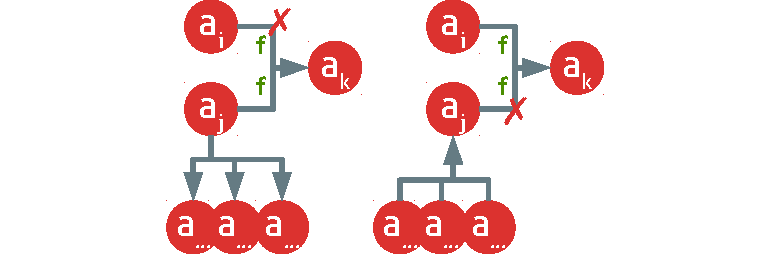
\includegraphics{graphics/competing.pdf}
\caption{Example of choice for cutting competing links based on
usefulness of actions\label{fig:competing}}
\end{figure}

In order to remove the least interesting link in competing causal links,
we need to compare their respective providing action to chose the most
useful ones.

\begin{definition}[Usefulness of an action]

The usefulness of an action is the number of participating links
(outgoing causal links) divided by the number of needing links (incoming
causal links). If there are no needing links, the usefulness is simmply
the number of participating links.

In the special cases if the action is either an initial step or a goal,
the usefulness is \(+\infty\). The usefulness of savior action is \(0\).

\end{definition}

We choose the link with the source action having the highest usefulness.
This replaces unnecessary savior actions and allows reducing the
usefulness of the least action in order to eventually make it an orphan
and prune it from the plan.

In the example figure \ref{fig:competing} the action \(a_j\) on the left
participates much more than the action \(a_i\) and therefore the link to
be removed would be \(a_i \xrightarrow{f} a_k\). On the right example
the actions doesn't have different outgoing links but the action \(a_j\)
is here much needier than its competitor and therefore the link to be
removed is the link \(a_j \xrightarrow{f} a_k\).

On the left example of figure \ref{fig:competing}, the action \(a_j\)
participates much more than the action \(a_i\) and therefore the link to
be removed would be \(a_i \xrightarrow{f} a_k\). On the right example
the actions don't have different outgoing links but the action \(a_j\)
is here much needier than its competitor. Therefore, the link to be
removed is the link \(a_j \xrightarrow{f} a_k\).

Actions can sometimes have no use in a plan as they don't contribute to
it.

\begin{definition}[Orphan actions]

Orphans actions are actions without any links or action with no outgoing
path to the goal (meaning that it doesn't participate in the plan). That
also concerns action that would become orphan if another orphan action
is removed.

\end{definition}

\begin{algorithm}\caption{Orphan actions finding}\label{orphanaction_find}\begin{algorithmic}[1]

\Function{$OrphanAction.$find}{Problem $P$} \State Actions
\(orphan \gets \emptyset\) \State int \(oldSize\) \Repeat
        \State \(oldSize \gets \#orphan\)
\ForAll{Action $step \in P.p.A_p$} \If{$step \in orphan$}
\State continue \EndIf
            \State int \(towardOrphan \gets 0\) \State Causal Links
\(outgoing \gets\) \protect\Call{outgoingEdgesOf}{$step$, $P.p$}
\ForAll{Causal Link $link \in outgoing$} \If{$link.target \in orphan$}
\State \(towardOrphan ++\) \EndIf
            \EndFor
            \If{$\#outgoing = towardOrphan \land step \notin \{ P.I, P.G\}$}
\State \(orphan \gets orphan \cup \{step\}\) \EndIf
        \EndFor
    \Until{$oldSize \neq \#orphan$} \State \Return \(orphan\)
\EndFunction

\end{algorithmic}\end{algorithm}

In order to fix this we derive the idea of the backward removal tree of
{[}4{]}. The algorithm, detailed in Algorithm 4, removes an action if
all its outgoing causal links are leading to useless actions. It
iterates over all actions until no new useless action is discovered. All
useless actions are then removed from the plan.

\begin{definition}[Competing actions]

In the same way links can be competing toward a common needer, there are
sometimes in the plan actions that are more suited to achieve a goal.
These actions are taken into account if they are more useful than the
source of the link, if they wouldn't cause a cycle and if they have
effects that are carried by the link.

\end{definition}

In such a case the link is removed and another one is formed by the
better suited action.

\subsection{Soft resolution}\label{soft-resolution}

\begin{algorithm}\caption{Soft resolution healing}\label{softresolution}\begin{algorithmic}[1]

\Function{heal}{Problem $P$} \State int \(minViolation \gets \infty\)
\State Plan \(best \gets P.p\) \State Flaw \(annoyer\)
\ForAll{$\langle flaw, plan \rangle \in P.partialSolutions$} \State int
\(currentViolation \gets\) \Call{violation}{$plan$, $P.G$}
\If{$currentViolation < minViolation$} \State \(best \gets plan\)
\State \(annoyer \gets flaw\)
\State \(minViolation \gets currentViolation\) \EndIf
    \EndFor
    \State \(P.p \gets best\)
\State \(P.partialSolutions \gets \emptyset\)
\ForAll{Resolver $resolver \in$ \Call{healers}{$annoyer$}}
\State \Call{apply}{$resolver$, $P.p$} \EndFor
\EndFunction

\end{algorithmic}\end{algorithm}

This auxiliary algorithm is meant to deal with failure. It will heal the
plan to make the failure recoverable for the next iteration of POP. Of
course it can't fix the plan by keeping the problem as it is. This
obviously breaks some properties as the algorithm no longer adheres to
the specification of the input, but in exchange it will always issue a
valid plan whatever happens. For more information on this property go
take a look at the \protect\hyperlink{hypersoundness}{appropriate
section bellow}.

Soft failure is useful when the precision and validity of the output is
not the most important criteria we look for. In some cases (like in
recognition processes) it is more useful to have an output even if it is
not exact than no output at all. That is why we propose a soft failing
mechanism for POP algorithms.

\subsubsection{Definitions}\label{definitions-1}

We define first some new notions, then we will explain the healing
algorithm.

\begin{definition}[Needer]

A needer is an action that needs a resolution related to a flaw. We
define different types of needer according to the type of the flaw.

\begin{itemize}
\item
  Subgoal needer For a subgoal \(a_n \xrightarrow{s} a_s\) the needer is
  the action \(a_n\) that has an unsatisfied precondition in the current
  partial plan.
\item
  Threat needer The needer of a threat \(a_t\) of a link
  \(a_p \xrightarrow{t} a_n\) is the target \(a_n\) of the threatened
  causal link.
\end{itemize}

\end{definition}

\begin{definition}[Proper fluents]

A proper fluent of a flaw is the one that caused the flaw. For a subgoal
\(a_n \xrightarrow{s} a_s\) it is the unsatisfied precondition \(s\).
For a threat \(a_t\) of a causal link \(a_p \xrightarrow{t} a_n\) it is
the fluent \(t\) held by the threatened causal link.

\end{definition}

\begin{definition}[Savior]

The savior of a flaw is the forged action
\(a_s = \langle \emptyset, \{p\} \rangle | a_s \notin A\) with \(p\)
being the proper fluent of the flaw.

\end{definition}

The concept of healer is made to target rogue flaws that caused total
failure.

\begin{definition}[Healers]

A healer is a resolver that is built around the savior of the flaw in
order to provide the missing fluents to it. The general formula of a
healer is the following : \[a_s \xrightarrow{p} a_n\] with \(a_s\) being
the savior of the flaw.

\end{definition}

For threats we need an additional healer specified as an ordering
constraint from the threatening action to the savior \(a_t \to a_s\) to
ensure that the savior acts after the threat and therefore provides the
proper fluent for the needer.

\begin{definition}[Violation degree]

The violation degree \(v(p)\) of a plan \(p\) is an indicator of the
health of a partial plan. It is the sum of the number of flaws and the
number of saviors in the plan.

\end{definition}

\subsubsection{Healing process}\label{healing-process}

The healing method is to keep track of reversions in the algorithm by
storing the partial plan and the unsatisfiable flaw each time a non
deterministic choice fails. We note the set of these failed plans \(F\).
As the POP algorithm encounters a final failure, this auxiliary
algorithm get invoked. The aim is to evaluate each backtracking partial
plan to choose the best one.

Therefore, we add an order relation for \(F\) noted
\[\prec : p \prec q \iff v(p) < v(q) | \{p, q\} \subset F\]

Once the POP algorithm fails completely, the soft failing algorithm can
be invoked to heal the plan. It chooses the best plan
\(b | \forall p \in F, b \prec p\) to heal it. If two plans have the
same violation degree, the algorithm chooses the first one to have
happened.

The healing process is similar to how POP works : we apply the healer of
the flaw that caused the failure of the partial plan we chosen. We empty
the set \(F\) to allow POP to iterate further since the flaw is
resolved. The healing process can be done for each unsolved flaws as POP
fails repeatedly. This ensures some interesting properties explained in
the following section.

\hypertarget{soda}{\section{SODA POP and its properties}\label{soda}}

The combination of classical POP and all the auxiliary algorithms
presented previously gives SODA POP algorithm detailed in Algorithm 6.
In this section we will focus on the properties of SODA POP.

\begin{algorithm}\caption{SODA POP}\label{soda}\begin{algorithmic}[1]

\Function{soda}{Problem $P$} \State \(P.p \gets\)
\Call{properPlan}{$P.G$, $P.A$} \Comment Offline execution then this
will be replaced by the previous online plan adjusted with the
environment. \State \Call{clean}{$P$} \State bool \(valid \gets false\)
\While{$\lnot valid$} \State \(valid \gets\) \Call{pop}{$P$}
\(= Success\) \If{$valid$} \State \Call{clean}{$P$}
\State \Return \(Success\) \EndIf
        \State \Call{heal}{$P$} \EndWhile
\EndFunction

\end{algorithmic}\end{algorithm}

\subsection{Convergence of POP}\label{convergence}

As to our knowledge, no proof of the convergence of POP has been done we
want to explicitly formulate one.

The classic planning problem is already proven to be decidable without
functions in the fluents {[}3{]}. Therefore, we can categorize the
termination cases.

\begin{proof}

In the case of a solvable problem, POP is proven to be complete. This
ensures that it will find a solution for the problem and therefore
terminate.

Be \(flaws(p)\) the set of flaws of a given partial plan. The number of
flaws is the number of subgoals plus the number of threats
\(flaws(p) = subgoals(p) \cup threats(p)\)

We consider the number of actions \(\#A\) as being finite. Therefore,
the number of steps in the plan is at worse \(\#A_p = \#A\). We also
assume that actions has a finite number of preconditions and effects
(since we don't use functions over fluents).

This leads to \(\#subgoals(p) < \sum_{a \in A_p} \#pre(a) < \infty\) and
\(\#threats(p) < \#L \le \sum_{a \in A_p} \#pre(a) < \infty\)

This means the number of all possible flaws is finite. As POP resolves
these flaws it will decrease their numbers and iterate over resolvers.
The number of resolver is \(\#subgoals(p) * \#A + \#threats(p) * 2\) and
is also finite. This means that the iteration will in the worst case be
of the number of resolvers before failing and this proves that the
algorithm terminates. \qedhere

\end{proof}

\subsection{Hypersoundness}\label{hypersoundeness}

Now that we proved that regular POP converges we can introduce the next
property : hyper soundness.

\begin{definition}[Hypersoundness]

An algorithm is said to be hypersound when it gives a valid solution for
all problems regardless of their resolvability.

\end{definition}

We note that this property isn't compatible with consistency regarding
the original problem and then doesn't fit the classical idea of
soundness that implicitly states that the validity of a solution is
relative to the problem. In the case of hypersoundness the problem is
valid and a solution to a problem \(P' = \langle A', I, G, p\rangle\).
We note the new set \(A' = A \cup S\) with \(S\) being the set of
saviors for all flaws that made the POP algorithm fails during the
execution of SODA.

The hypersoundness of our combined algorithm is proven using the
convergence of POP and the way the Soft solving behaves.

\begin{proof}[Hypersoundness of SODA POP]

The proper plan and defect fixing algorithms are obviously convergent.
The proper plan algorithm cannot iterate more than the number of actions
(since duplicates are forbidden) and the defect resolution will fix the
finite numbers of defects present in the finite partial plan issued by
the proper plan algorithm.

POP is sound and converges. Therefore, if SODA POP converges it will
return a valid solution for \(P'\). In the same way we proved for POP,
the new healing process converges because it reduces the number of flaws
in the partial plan and since this number is finite, the algorithm
converges.\qedhere

\end{proof}

\subsection{Enhancement for online
planning}\label{enhancement-for-online-planning}

SODA POP algorithm can be used in dynamic online environments to allow a
robust way to replan an existing obsolete plan. The first thing to
execute prior to the runtime is the generation of the proper plans for
all the goals that will be considered.

For the first execution of the online planning the initial state is
added to the problem and the defect detection is applied with the rest
of the SODA POP algorithm. This will give the first plan.

For every change of the environment the previous plan is modified
accordingly and then fed to the defect detection and SODA algorithm
again. This must be done each time the plan is modified in order to
actualize the plan. The new plan will have all defects fixed. For
example a savior action can be removed if the initial step or a new
action becomes competing with it and actions with liar link to a removed
fluent in the goal will become probably an orphan.

In practice this will generate little to no iteration of the algorithm.

\section{Experimental results}\label{experimental-results}

In order to test the validity of these algorithms we implemented a
prototype in Java. This prototype is exactly derived from the
definitions and pseudo code presented in this paper. We used basic
actions with integer fluents to focus on the way the algorithm behaves.

For the simulation runs we used a computer with an Intel® Core™
i7-4720HQ CPU clocking at 2.60GHz for 8 cores and 8GB of memory. The
speed was measured in nano seconds before and after the call to the
solve function. The process has a warming up phase that compute random
plans for a few seconds before starting the benchmarks. The computer was
left idle during the test to remove any related noise to the
measurements.

\subsection{Quality of classical POP}\label{quality-of-classical-pop}

The first metric we decided to measure was the performance of our
reference POP algorithm. We measured the solving time for valid problems
and the quality of the resulting plans. In figure \ref{fig:quality} we
can see a plot of these measures.

\begin{figure}[htbp]
\centering
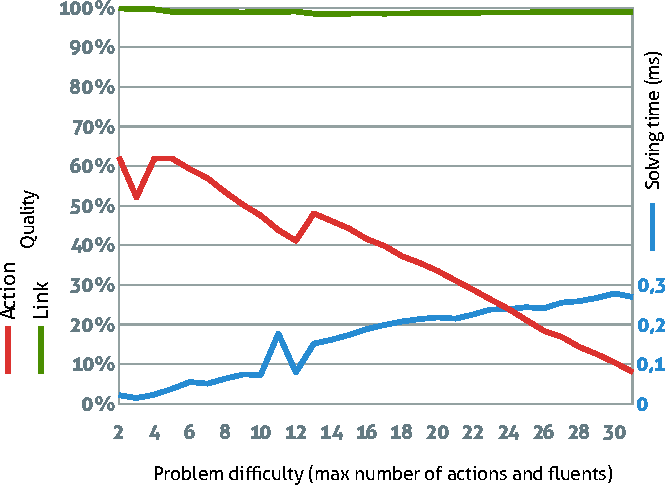
\includegraphics{graphics/quality.pdf}
\caption{Action and link quality and solving time of POP over \(10 000\)
valid problems for each difficulty\label{fig:quality}}
\end{figure}

We tested the algorithm with randomly generated valid problems. We
generated those by randomly creating plans based on a difficulty setting
that was the upper bound for the number of actions and half the possible
number of fluents. This difficulty setting also made the initial and
goal step larger accordingly. The actions were cleaned of any toxicity
and was built using a forward chaining algorithm. We added also random
unrelated actions. Each problem was verified by POP before being
generated to ensure resolvability.

As we clearly see in the figure \ref{fig:quality}, POP linearly increase
its solving time depending on the problem difficulty. That obviously
follows the fact that POP has more flaws to fix and therefore more
iterations.

As we can observe, POP has a rather high link quality with almost no
problems issued with causal link regardless of the difficulty of the
problem. This can be linked to either the way we generated our valid
plans or to a real tendency of POP to not create that kind of defects on
its own.

The action quality on the other hand drops significantly as the
difficulty gets higher. This is linked to the number of competing and
useless actions that can make the plan simpler but are kept by the flaw
selection mechanism of POP.

\subsection{Performance of SODA POP}\label{performance-of-soda-pop}

As SODA POP and regular POP doesn't have the same range of capabilities
we can't compare them hand to hand. Indeed, our algorithm will always
output plans with 100\% quality since the defect detection system aims
to remove them all and since our algorithms is hypersound it will give
valid plans for unsolvable problems by derivation. In these case POP
won't be able to return a result and will terminate much quicker as the
plan is found unsolvable.

Therefore, we measured the performances of our set of algorithms on
completely random problems. Each time the algorithm outputted a solution
with the lowest possible violation despite the complete invalidity of
the input. In figure \ref{fig:performance} we can see the way SODA POP
scales up on larger problems.

\begin{figure}[htbp]
\centering
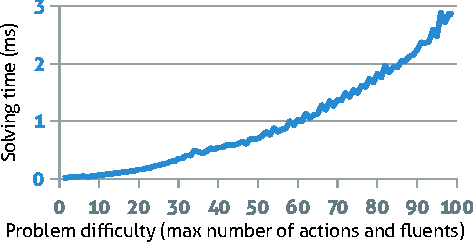
\includegraphics{graphics/performance.pdf}
\caption{Average solving time of SODA POP over \(10 000\) random
problems for each difficulty\label{fig:performance}}
\end{figure}

The performances display logarithmic solving time. This is explained by
the fact that POP has to be called recursively on the healed problems.
The defect detection participates too in the increase of solving time
especially the competing action detection that needs to iterate over all
actions and edges and calculate usefulness for two actions each time.

\section*{Conclusion}\label{conclusion}
\addcontentsline{toc}{section}{Conclusion}

We defined our SODA POP algorithm and demonstrated its properties. The
set of algorithms has extended capabilities of plan repairing and soft
solving as shown in examples and simulations. While slower than POP, the
resilience of SODA POP can be used in various applications. We aim to
use it on the particular case of online plan recognition and decision
making as the capabilities to derive plans and repair them will prove
useful when comparing potential goals with observed plans.

The algorithm can be improved with a better defect detection algorithm
that can rank them and start fixing the most offensive defects before
targeting others. Also, if the competing action detection can be
improved, it can be used as heuristic for resolver selection to improve
the performances.

Another way the present work can be improved is by extending it to the
use of more expressive fluents and port all notions to variable choices.
One possible goal would be to combine this work with ontologies or an
argumentation language in order to significantly boost expressiveness.

We hope that this work will be useful and that it will be extended and
used in various applications in the future and that is why we plan to
release the software with an open source license soon.

\section*{References}\label{references}
\addcontentsline{toc}{section}{References}

\hypertarget{refs}{}
\hypertarget{ref-weldux5fintroductionux5f1994}{}
{[}1{]} D. S. Weld, ``An introduction to least commitment planning,''
\emph{AI magazine}, vol. 15, no. 4, p. 27, 1994.

\hypertarget{ref-richterux5flamaux5f2011}{}
{[}2{]} S. Richter, M. Westphal, and M. Helmert, ``LAMA 2008 and 2011,''
in \emph{International Planning Competition}, 2011, pp. 117--124.

\hypertarget{ref-ghallabux5fautomatedux5f2004}{}
{[}3{]} M. Ghallab, D. S. Nau, and P. Traverso, \emph{Automated
planning: theory and practice}. Amsterdam ; Boston: Elsevier/Morgan
Kaufmann, 2004.

\hypertarget{ref-vanux5fderux5fkrogtux5fplanux5f2005}{}
{[}4{]} R. Van Der Krogt and M. De Weerdt, ``Plan Repair as an Extension
of Planning.'' in \emph{ICAPS}, 2005, vol. 5, pp. 161--170.

\hypertarget{ref-ramirezux5fplanux5f2009}{}
{[}5{]} M. Ramırez and H. Geffner, ``Plan recognition as planning,'' in
\emph{Proceedings of the 21st international joint conference on
Artifical intelligence. Morgan Kaufmann Publishers Inc}, 2009, pp.
1778--1783.

\hypertarget{ref-erolux5fumcp:ux5f1994}{}
{[}6{]} K. Erol, J. A. Hendler, and D. S. Nau, ``UMCP: A Sound and
Complete Procedure for Hierarchical Task-network Planning.'' in
\emph{AIPS}, 1994, vol. 94, pp. 249--254.

\hypertarget{ref-penberthyux5fucpop:ux5f1992}{}
{[}7{]} J. S. Penberthy, D. S. Weld, and others, ``UCPOP: A Sound,
Complete, Partial Order Planner for ADL.'' \emph{Kr}, vol. 92, pp.
103--114, 1992.

\hypertarget{ref-bechonux5fhipop:ux5f2014}{}
{[}8{]} P. Bechon, M. Barbier, G. Infantes, C. Lesire, and V. Vidal,
``HiPOP: Hierarchical Partial-Order Planning,'' in \emph{STAIRS 2014:
Proceedings of the 7th European Starting AI Researcher Symposium}, 2014,
vol. 264, p. 51.

\hypertarget{ref-garciaux5fdefeasibleux5f2008}{}
{[}9{]} D. R. García, A. J. García, and G. R. Simari, ``Defeasible
reasoning and partial order planning,'' in \emph{Foundations of
Information and Knowledge Systems}, Springer, 2008, pp. 311--328.

\hypertarget{ref-colesux5fforward-chainingux5f2010}{}
{[}10{]} A. J. Coles, A. Coles, M. Fox, and D. Long, ``Forward-Chaining
Partial-Order Planning.'' in \emph{ICAPS}, 2010, pp. 42--49.

\end{document}
